\subsubsection{User-management}

\begin{center}
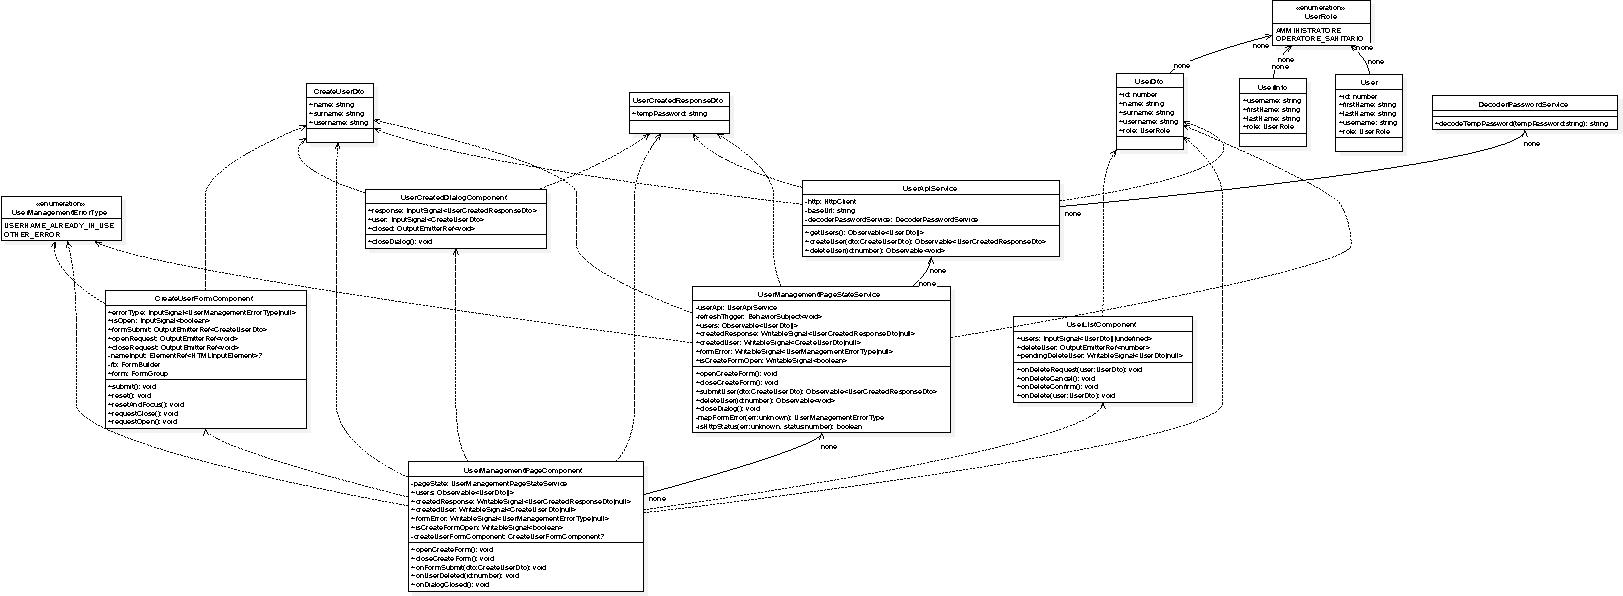
\includegraphics[width=\textwidth]{./frontend/user-management/user-management.pdf}
\captionof{figure}{Diagramma delle classi del modulo User management}
\end{center}


\addAtr{+}{errorType: InputSignal$<$UserManagementErrorType $|$ null$>$}{Segnale di input che trasporta l'eventuale tipo di errore da visualizzare nel form.}
\addAtr{+}{isOpen: InputSignal$<$boolean$>$}{Segnale di input che indica se il form è attualmente aperto.}
\addAtr{+}{formSubmit: OutputEmitterRef$<$CreateUserDto$>$}{Evento emesso al submit del form, contenente i dati dell'utente da creare.}
\addAtr{+}{openRequest: OutputEmitterRef$<$void$>$}{Evento emesso quando il componente richiede di essere aperto.}
\addAtr{+}{closeRequest: OutputEmitterRef$<$void$>$}{Evento emesso quando il componente richiede di essere chiuso.}
\addAtr{-}{nameInput?: ElementRef$<$HTMLInputElement$>$}{Riferimento al campo di input del nome, utilizzato per il focus automatico dopo il reset.}
\addAtr{-}{fb: FormBuilder}{Istanza di \texttt{FormBuilder} utilizzata per la costruzione del form reattivo.}
\addAtr{+}{form: FormGroup}{Form reattivo contenente i campi \texttt{name}, \texttt{surname} e \texttt{username} con i relativi validatori.}
\addMet{+}{submit() : void}{Emette i dati del form se valido, altrimenti marca tutti i campi come toccati per mostrare gli errori di validazione.}
\addMet{+}{reset() : void}{Reimposta tutti i campi del form ai valori vuoti iniziali.}
\addMet{+}{resetAndFocus() : void}{Reimposta il form, ne ripristina lo stato pristine e untouched, e sposta il focus sul campo del nome.}
\addMet{+}{requestClose() : void}{Emette l'evento \texttt{closeRequest} per segnalare la richiesta di chiusura del form.}
\addMet{+}{requestOpen() : void}{Emette l'evento \texttt{openRequest} per segnalare la richiesta di apertura del form.}
\makeCl{CreateUserFormComponent}{Componente Angular che gestisce il form reattivo per la creazione di un nuovo utente. Espone segnali di input per lo stato e gli errori, ed eventi di output per le azioni di submit, apertura e chiusura.}

\addAtr{+}{response: InputSignal$<$UserCreatedResponseDto$>$}{Segnale di input obbligatorio contenente i dati di risposta restituiti dopo la creazione dell'utente.}
\addAtr{+}{user: InputSignal$<$CreateUserDto$>$}{Segnale di input obbligatorio contenente i dati dell'utente appena creato.}
\addAtr{+}{closed: OutputEmitterRef$<$void$>$}{Evento emesso quando l'utente chiude il dialog.}
\addMet{+}{closeDialog() : void}{Emette l'evento \texttt{closed} per segnalare la chiusura del dialog.}
\makeCl{UserCreatedDialogComponent}{Componente Angular che visualizza un dialog di conferma al termine della creazione di un utente. Viene mostrato solo quando i dati di risposta e dell'utente sono disponibili, grazie all'uso di input obbligatori.}

\addAtr{+}{users: InputSignal$<$UserDto[]$>$}{Segnale di input contenente la lista degli utenti da visualizzare.}
\addAtr{+}{deleteUser: OutputEmitterRef$<$number$>$}{Evento emesso alla conferma dell'eliminazione, contenente l'id dell'utente da eliminare.}
\addAtr{+}{pendingDeleteUser: WritableSignal$<$UserDto $|$ null$>$}{Segnale che mantiene l'utente in attesa di conferma di eliminazione, o \texttt{null} se nessuna eliminazione è in corso.}
\addMet{+}{onDeleteRequest(user: UserDto) : void}{Imposta l'utente specificato come candidato all'eliminazione, avviando il flusso di conferma.}
\addMet{+}{onDeleteCancel() : void}{Annulla l'eliminazione in corso reimpostando il segnale \texttt{pendingDeleteUser} a \texttt{null}.}
\addMet{+}{onDeleteConfirm() : void}{Conferma l'eliminazione dell'utente in attesa, emette l'evento \texttt{deleteUser} con il suo id e reimposta il segnale a \texttt{null}.}
\addMet{+}{onDelete(user: UserDto) : void}{Gestisce la richiesta di eliminazione di un utente delegando a \texttt{onDeleteRequest}.}
\makeCl{UserListComponent}{Componente Angular che visualizza la lista degli utenti e gestisce il flusso di eliminazione con richiesta di conferma. Utilizza un segnale interno per tracciare l'utente in attesa di eliminazione prima di emettere l'evento definitivo.}

\addAtr{-}{pageState: UserManagementPageStateService}{Servizio di stato della pagina, utilizzato per coordinare tutte le operazioni di gestione utenti.}
\addAtr{+}{users\$: Observable$<$UserDto[]$>$}{Stream reattivo contenente la lista aggiornata degli utenti da visualizzare.}
\addAtr{+}{createdResponse: Signal$<$UserCreatedResponseDto $|$ null$>$}{Segnale contenente la risposta dell'ultima operazione di creazione utente, o \texttt{null} se non disponibile.}
\addAtr{+}{createdUser: Signal$<$CreateUserDto $|$ null$>$}{Segnale contenente i dati dell'ultimo utente creato, utilizzato per la visualizzazione nel dialog di conferma.}
\addAtr{+}{formError: Signal$<$UserManagementErrorType $|$ null$>$}{Segnale contenente l'eventuale tipo di errore da mostrare nel form di creazione.}
\addAtr{+}{isCreateFormOpen: Signal$<$boolean$>$}{Segnale che indica se il form di creazione utente è attualmente aperto.}
\addAtr{-}{createUserFormComponent?: CreateUserFormComponent}{Riferimento al componente del form di creazione, utilizzato per il reset e il focus dopo una creazione avvenuta con successo.}
\addMet{+}{openCreateForm() : void}{Delega al servizio di stato l'apertura del form di creazione utente.}
\addMet{+}{closeCreateForm() : void}{Delega al servizio di stato la chiusura del form di creazione utente.}
\addMet{+}{onFormSubmit(dto: CreateUserDto) : void}{Invia i dati del form al servizio di stato e, in caso di successo, reimposta il focus sul form.}
\addMet{+}{onUserDeleted(id: number) : void}{Delega al servizio di stato l'eliminazione dell'utente con l'id specificato.}
\addMet{+}{onDialogClosed() : void}{Delega al servizio di stato la chiusura del dialog di conferma creazione.}
\makeCl{UserManagementPageComponent}{Componente Angular che funge da pagina principale per la gestione degli utenti, orchestrando i sottocomponenti di lista, form di creazione e dialog di conferma. Delega tutta la logica di stato al servizio UserManagementPageStateService.}

\addAtr{+}{tempPassword: string}{}
\makeAbCl{UserCreatedResponseDto}{Interfaccia che rappresenta la risposta minima restituita dal backend alla creazione di un utente. Espone esclusivamente la password temporanea assegnata all'utente appena creato.}

\addAtr{+}{id: number}{}
\addAtr{+}{name: string}{}
\addAtr{+}{surname: string}{}
\addAtr{+}{username: string}{}
\addAtr{+}{role: UserRole}{}
\makeAbCl{UserDto}{Interfaccia che rappresenta i dati di un utente restituiti dal backend nelle chiamate GET. Raccoglie le informazioni anagrafiche e il ruolo dell'utente.}

\addAtr{+}{name: string}{}
\addAtr{+}{surname: string}{}
\addAtr{+}{username: string}{}
\makeAbCl{CreateUserDto}{Interfaccia che rappresenta i dati necessari per la creazione di un nuovo utente. Raccoglie le informazioni anagrafiche e il nome utente da inviare al backend.}

\addAtr{+}{username: string}{}
\addAtr{+}{firstName: string}{}
\addAtr{+}{lastName: string}{}
\addAtr{+}{role: UserRole}{}
\makeAbCl{UserInfo}{Interfaccia che rappresenta le informazioni di base di un utente autenticato. Raccoglie nome utente, dati anagrafici e ruolo.}

\addAtr{+}{id: number}{}
\addAtr{+}{firstName: string}{}
\addAtr{+}{lastName: string}{}
\addAtr{+}{username: string}{}
\addAtr{+}{role: UserRole}{}
\makeAbCl{User}{Interfaccia che rappresenta il modello di dominio di un utente. Raccoglie le informazioni anagrafiche, il nome utente e il ruolo assegnato.}


\addMet{+}{decodeTempPassword(tempPassword: string) : string}{Decodifica una password temporanea da Base64, restituendo la stringa originale se il valore non è un Base64 valido o se la decodifica fallisce.}
\makeCl{DecoderPasswordService}{Servizio Angular per la decodifica delle password temporanee codificate in Base64. Verifica preventivamente che la stringa rispetti il formato Base64 prima di tentare la decodifica.}

\addAtr{-}{http: HttpClient}{Client HTTP utilizzato per effettuare le richieste alle API REST.}
\addAtr{-}{baseUrl: string}{URL base dell'API, iniettato tramite token \texttt{API\_BASE\_URL}.}
\addAtr{-}{decoderPasswordService: DecoderPasswordService}{Servizio utilizzato per decodificare la password temporanea restituita dal backend.}
\addMet{+}{getUsers() : Observable$<$UserDto[]$>$}{Recupera la lista completa degli utenti tramite una richiesta GET al backend.}
\addMet{+}{createUser(dto: CreateUserDto) : Observable$<$UserCreatedResponseDto$>$}{Invia una richiesta POST per la creazione di un nuovo utente e decodifica la password temporanea contenuta nella risposta.}
\addMet{+}{deleteUser(id: number) : Observable$<$void$>$}{Invia una richiesta DELETE per eliminare l'utente con l'id specificato.}
\makeCl{UserApiService}{Servizio Angular per la comunicazione con le API REST relative alla gestione degli utenti. Espone operazioni di lettura, creazione ed eliminazione utenti, gestendo la decodifica della password temporanea restituita alla creazione.}

\addAtr{-}{userApi: UserApiService}{Servizio utilizzato per effettuare le chiamate API relative agli utenti.}
\addAtr{-}{refreshTrigger\$: BehaviorSubject$<$void$>$}{Subject utilizzato per innescare il ricaricamento della lista utenti.}
\addAtr{+}{users\$: Observable$<$UserDto[]$>$}{Stream reattivo che emette la lista aggiornata degli utenti ad ogni refresh, restituendo un array vuoto in caso di errore.}
\addAtr{+}{createdResponse: WritableSignal$<$UserCreatedResponseDto $|$ null$>$}{Segnale contenente la risposta dell'ultima operazione di creazione utente, o \texttt{null} se il dialog è chiuso.}
\addAtr{+}{createdUser: WritableSignal$<$CreateUserDto $|$ null$>$}{Segnale contenente i dati dell'ultimo utente creato, o \texttt{null} se il dialog è chiuso.}
\addAtr{+}{formError: WritableSignal$<$UserManagementErrorType $|$ null$>$}{Segnale contenente l'eventuale tipo di errore verificatosi durante la creazione utente.}
\addAtr{+}{isCreateFormOpen: WritableSignal$<$boolean$>$}{Segnale che indica se il form di creazione utente è attualmente aperto.}
\addMet{+}{openCreateForm() : void}{Imposta il segnale \texttt{isCreateFormOpen} a \texttt{true} per aprire il form di creazione.}
\addMet{+}{closeCreateForm() : void}{Imposta il segnale \texttt{isCreateFormOpen} a \texttt{false} per chiudere il form di creazione.}
\addMet{+}{submitUser(dto: CreateUserDto) : Observable$<$UserCreatedResponseDto$>$}{Invia i dati del nuovo utente all'API, aggiorna i segnali di stato e innesca il refresh della lista in caso di successo.}
\addMet{+}{deleteUser(id: number) : Observable$<$void$>$}{Elimina l'utente con l'id specificato tramite l'API e innesca il refresh della lista in caso di successo.}
\addMet{+}{closeDialog() : void}{Reimposta i segnali \texttt{createdResponse} e \texttt{createdUser} a \texttt{null} per chiudere il dialog di conferma.}
\addMet{-}{mapFormError(err: unknown) : UserManagementErrorType}{Mappa un errore HTTP nel corrispondente tipo di errore del form, distinguendo il caso di username già in uso dagli altri errori.}
\addMet{-}{isHttpStatus(err: unknown, status: number) : err is \{status: number\}}{Verifica se l'errore fornito è un oggetto con il codice di stato HTTP specificato.}
\makeCl{UserManagementPageStateService}{Servizio di stato per la pagina di gestione utenti, responsabile del coordinamento tra le chiamate API e i segnali reattivi esposti ai componenti. Gestisce il ciclo di vita delle operazioni di creazione, eliminazione e refresh della lista utenti.}